\section{Introduction} \label{sec:introduction}
    \IEEEPARstart{R}{espiratory} motion reduces image resolution in \gls{PET} by introducing blurring \& mis-alignment artefacts~\cite{Nehmeh2008a}. 

\section{Methods} \label{sec:methods}
\subsection{Data Acquisition} \label{sec:data_acquisition}
        Seven dynamic \gls{FDG} acquisitions, with a \gls{FOV} covering the upper lung \& heart, were acquired on a \gls{GE} Discovery $710$. Each acquisition lasted approximately \SI{20}{\minute} with the acquisition starting before injection of the radiotracer. \gls{SS} were acquired in parallel using a \gls{RPM}.
        
    \subsection{Data Preparation} \label{sec:data_preparation}
        Data were unlisted into low resolution sinograms, at a time interval of \SI{500}{\milli\second}, using the \gls{GE} PetToolbox following~\cite{Bertolli2018Data-DrivenTomography}. Data was preprocessed by removing the first \& last element in the axial direction and applying a Freeman-Tukey to stabilise the variance of the Poisson data. The Freeman-Tukey transformation is defined as:
        
        \begin{equation}
            S = 2 \sqrt{S + \frac{3}{8}}
        \end{equation}
        
        \noindent $S$ is the resultant sinogram of applying the Freeman-Tukey transformation to sinogram $S$~\cite{Freeman1950TransformationsRoot}.
    
    \subsection{Surrogate Signal Extraction} \label{sec:surrogate_signal_extraction}
        \subsubsection{Moving Window} \label{sec:moving_window}
            This method takes data window by window (with half a window overlap) \& extracts a \gls{SS} using \gls{PCA}. The final \gls{SS} is constructed by determining the sign of the current \gls{SS}, flipping it if necessary, and then concatenating it with the next. The size of the window increases as the acquisition goes on. Motivation is that at early time points the variation caused by the tracer kinetics obscures that which comes from respiratory motion, if the window is smaller than the period of the tracer kinetics then it should obtain the respiratory \gls{SS}.
        
        \subsubsection{One \gls{PC}} \label{sec:one_pc}
            This method takes late time point \glss{PC} \& applies them to early time point data. Motivation is that the \glss{PC} of late time point data do not vary significantly, therefore it could be assumed that the variation of early time point \glss{PC} are caused mostly by the tracer kinetics.
        
        \subsubsection{Joint Method} \label{sec:joint_method}
            This method attempts to take the advantages of both the one \gls{PC} method and the static method, by truncating \& concatenating the result of the start of one with the end of the other. Motivation is that the static method would work better on static data, once the tracer kinetics have subsided the acquisition could be considered to be static.
    
    
    \subsection{Evaluation} \label{sec:evaluation}
        \subsubsection{Cross Correlation} \label{sec:cross_correlation}
            The \gls{CC} of each \gls{SS} between each method and the \gls{RPM}, for all acquisitions, has been calculated. Additionally, the early time point \glss{SS} for each method have been plotted against the \gls{RPM}, for the first acquisition.
        
        \subsubsection{Reconstruction} \label{sec:reconstruction}
            Data has been reconstructed, for the first acquisition, using each \gls{SS} to displacement gate the data into $10$ bins. Reconstructions were performed using \gls{GE} Duetto using \gls{TOF} \gls{OSEM} with two full iterations \& $24$ subsets.%~\cite{Hudson1994}.
            Volumes were post-filtered using a Gaussian blur with a kernel size of \SI{6.4}{\milli\metre} \gls{FWHM}.
            
            Comparisons between these \gls{MC} reconstructed volumes includes: A profile over the aorta \& \gls{SUV}\textsubscript{max}, \gls{SUV}\textsubscript{median} \& \gls{SUV}\textsubscript{peak}. \gls{SUV}\textsubscript{peak} here was defined following \gls{EANM} guidelines.%~\cite{Boellaard2015FDG2.0}
        
\section{Results} \label{sec:results}
    \begin{table}
        \centering
        \captionsetup{singlelinecheck=false, justification=centering}
        \caption{A comparison of the \gls{CC} between the \gls{RPM} \gls{SS} \& the \gls{SS} from the static \gls{PCA}, the moving window, the one \gls{PC} \& the joint methods for $7$ acquisitions.}
        
        \resizebox*{0.75\linewidth}{!}
        {
            \begin{tabular}{||c|cccc||}
                \hline
                \textbf{\gls{CC}} & \textbf{Static \gls{PCA}} & \textbf{Moving Window} & \textbf{One \gls{PC}} & \textbf{Joint Method} \\
                \hline
                \textbf{Acquisition $1$}   & $0.0387$  & $0.486$  & $0.565$  & $0.493$   \\
                \textbf{Acquisition $2$}   & $0.0985$  & $0.0361$ & $0.281$  & $0.0227$  \\
                \textbf{Acquisition $3$}   & $0.00797$ & $0.0388$ & $0.224$  & $0.00459$ \\
                \textbf{Acquisition $4$}   & $0.242$   & $0.0467$ & $0.273$  & $0.0946$  \\
                \textbf{Acquisition $5$}   & $0.0759$  & $0.793$  & $0.819$  & $0.798$   \\
                \textbf{Acquisition $6$}   & $0.0594$  & $0.246$  & $0.363$  & $0.259$   \\
                \textbf{Acquisition $7$}   & $0.160$   & $0.629$  & $0.203$  & $0.526$   \\
                \hline
            \end{tabular}
        }
        \label{tab:cross_correlation}
    \end{table}
    
    A comparison of \gls{CC} can be seen in in~\Fref{tab:cross_correlation}. The results for the moving window method show that it usually performs better than static \gls{PCA}, a reason why these results may be varied is because the hyper parameters for this method were optimised for one acquisition. The results for the one \gls{PC} method are consistently better than the static \gls{PCA} method.
    
    \begin{figure}
        \centering
        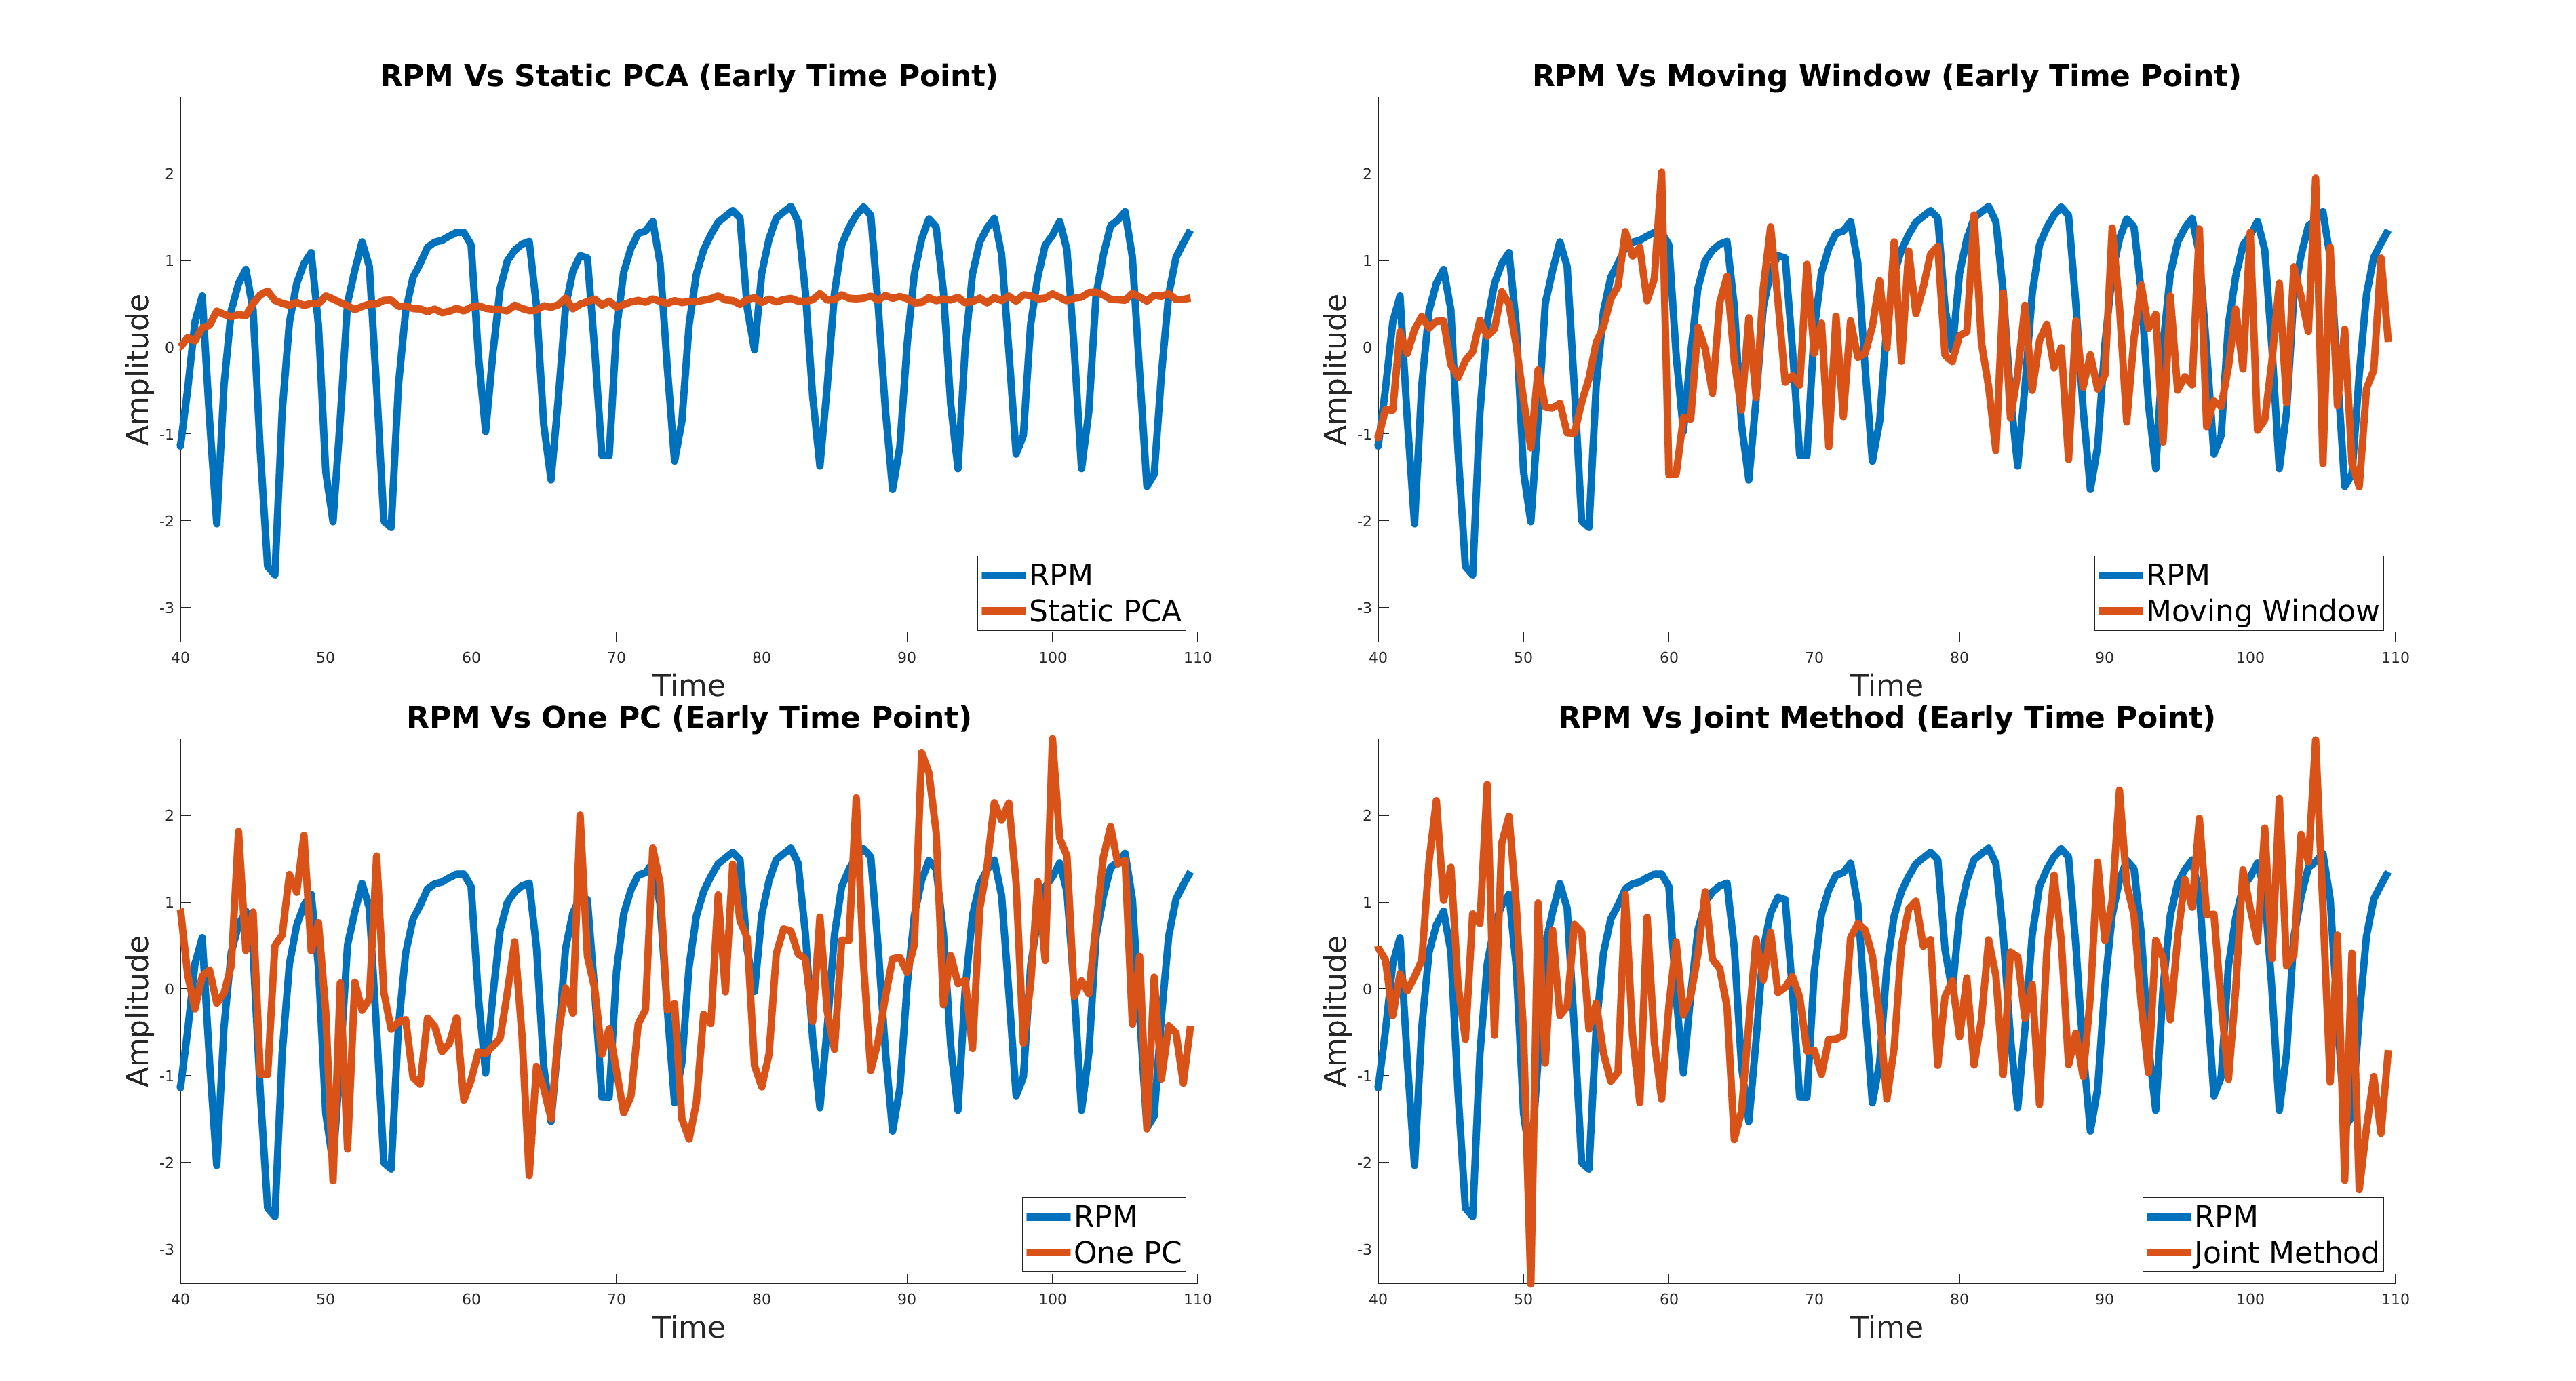
\includegraphics[width=1.0\linewidth]{figures/surrogate_signal.png}
        \captionsetup{singlelinecheck=false, justification=centering}
        \caption{A comparison between the \gls{RPM} \gls{SS} \& the \gls{SS} from the static \gls{PCA}, the moving window, the one \gls{PC} \& the joint methods.}
        \label{fig:surrogate_signal}
    \end{figure}
    
    \begin{figure}
        \centering
        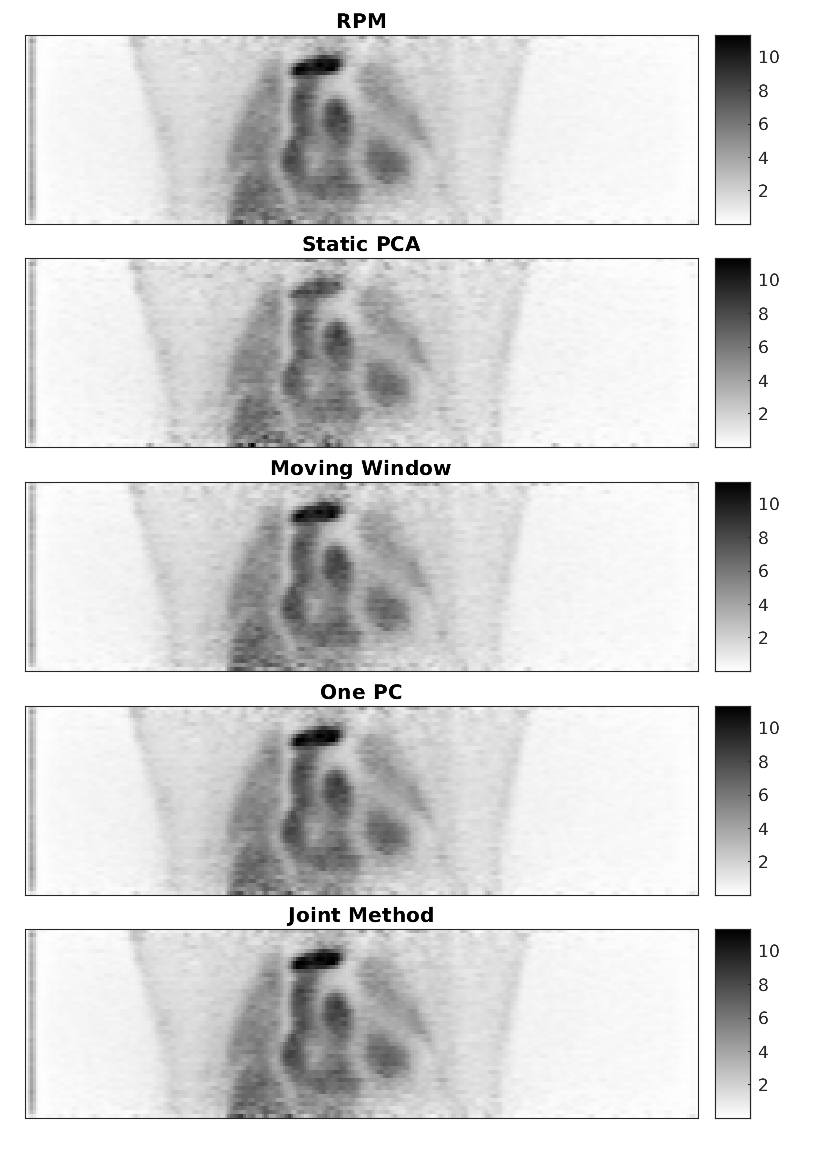
\includegraphics[width=0.75\linewidth]{figures/visual_analysis_pca.png}
        \captionsetup{singlelinecheck=false, justification=centering}
        \caption{Gated reconstructions using \gls{RPM}, static \gls{PCA} method, moving window method, one \gls{PC} method \& joint method. Colour map ranges are consistent for all images.}
        \label{fig:visual_analysis}
    \end{figure}
    
    \begin{figure}
        \centering
        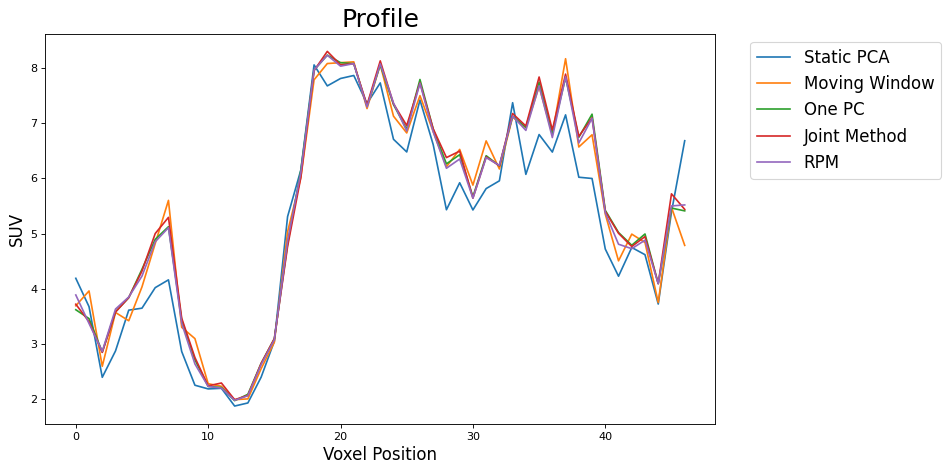
\includegraphics[width=0.5\linewidth]{figures/profile_pca.png}
        \captionsetup{singlelinecheck=false, justification=centering}
        \caption{A profile across the aorta for gated reconstructions using \gls{RPM}, static \gls{PCA} method, moving window method, one \gls{PC} method \& joint method.}
        \label{fig:profile}
    \end{figure}
    
    \begin{table}
        \centering
        \captionsetup{singlelinecheck=false, justification=centering}
        \caption{Comparison of \gls{SUV}\textsubscript{max}, \gls{SUV}\textsubscript{median} \& \gls{SUV}\textsubscript{peak} between gated reconstructions using \gls{RPM}, static \gls{PCA} method, moving window method, one \gls{PC} method \& joint method.}
        
        \resizebox*{0.5\linewidth}{!}
        {
            \begin{tabular}{||c|ccc||}
                \hline
                \textbf{\gls{SUV}} & \textbf{Max} & \textbf{Median} & \textbf{Peak} \\
                \hline
                \textbf{\gls{RPM}}          & $18.4$ & $10.9$ & $12.6$ \\
                \hline
                \textbf{Static \gls{PCA}}   & $12.8$ & $10.6$ & $11.4$ \\
                \textbf{Moving Window}      & $14.5$ & $10.6$ & $11.3$ \\
                \textbf{One \gls{PC}}       & $18.5$ & $10.9$ & $12.6$ \\
                \textbf{Joint Method}       & $18.5$ & $11.0$ & $12.8$ \\
                \hline
            \end{tabular}
        }
        \label{tab:suv}
    \end{table}
    
    A plot of the \gls{SS} for all methods can be seen in~\Fref{fig:surrogate_signal}, the one \gls{PC} method matches the \gls{RPM} best in this example. The reconstructed data, using \glss{SS} from all methods can be seen in~\Fref{fig:visual_analysis}. The clarity of the reconstruction around the aorta seems diminished in the static \gls{PCA} example, it is similar in all other examples. A profile across the aorta can be seen in~\Fref{fig:profile}, this shows that the static \gls{PCA} method differs in its distribution compared to the others. \gls{SUV} results can be seen in~\Fref{tab:suv} \& show that \glss{SUV} are consistent with \gls{RPM} for both the one \gls{PC} method and the joint method.
    
\section{Discussion \& Conclusions} \label{sec:discussion_and_conclusions}
    
